\documentclass[fleqn]{article}

%% Created with wxMaxima 25.01.0

\setlength{\parskip}{\medskipamount}
\setlength{\parindent}{0pt}
\usepackage{iftex}
\ifPDFTeX
  % PDFLaTeX or LaTeX 
  \usepackage[utf8]{inputenc}
  \usepackage[T1]{fontenc}
  \DeclareUnicodeCharacter{00B5}{\ensuremath{\mu}}
\else
  %  XeLaTeX or LuaLaTeX
  \usepackage{fontspec}
\fi
\usepackage{graphicx}
\usepackage{color}
\usepackage[leqno]{amsmath}
\usepackage{ifthen}
\newsavebox{\picturebox}
\newlength{\pictureboxwidth}
\newlength{\pictureboxheight}
\newcommand{\includeimage}[1]{
    \savebox{\picturebox}{\includegraphics{#1}}
    \settoheight{\pictureboxheight}{\usebox{\picturebox}}
    \settowidth{\pictureboxwidth}{\usebox{\picturebox}}
    \ifthenelse{\lengthtest{\pictureboxwidth > .95\linewidth}}
    {
        \includegraphics[width=.95\linewidth,height=.80\textheight,keepaspectratio]{#1}
    }
    {
        \ifthenelse{\lengthtest{\pictureboxheight>.80\textheight}}
        {
            \includegraphics[width=.95\linewidth,height=.80\textheight,keepaspectratio]{#1}
            
        }
        {
            \includegraphics{#1}
        }
    }
}
\newlength{\thislabelwidth}
\DeclareMathOperator{\abs}{abs}

\definecolor{labelcolor}{RGB}{100,0,0}

\begin{document}


\noindent
%%%%%%%%
%% INPUT:
\begin{minipage}[t]{4.000000em}\color{red}\bfseries
(\% i63)	
\end{minipage}
\begin{minipage}[t]{\textwidth}\color{blue}
f(x):=(3*x+15*x\^\ 2-x\^\ 4)/(9*x\^\ 2+1);
\end{minipage}
%%%% OUTPUT:
\[\displaystyle \tag{\% o63} 
\mathop{f}(x)\mathop{:=}\frac{3 x\mathop{+}15 {{x}^{2}}\mathop{-}{{x}^{4}}}{9 {{x}^{2}}\mathop{+}1}\mbox{}
\]
%%%%%%%%%%%%%%%%


\noindent
%%%%%%%%
%% INPUT:
\begin{minipage}[t]{4.000000em}\color{red}\bfseries
(\% i65)	
\end{minipage}
\begin{minipage}[t]{\textwidth}\color{blue}
float(solve(f(x)=0));
\end{minipage}
%%%% OUTPUT:
\[\displaystyle \tag{\% o65} 
\mathop{[}x\mathop{=}\left( \mathop{-}\left( 0.866 \% i\right) \mathop{-}0.5\right)  {{\left( 11.1 \% i\mathop{+}1.5\right) }^{\frac{1}{3}}}\mathop{+
}\frac{5.0 \left( 0.866 \% i\mathop{-}0.5\right) }{{{\left( 11.1 \% i\mathop{+}1.5\right) }^{\frac{1}{3}}}}\mathop{,}x\mathop{=}\left( 0.866 \% i\mathop{-}0.5\right) {{\left( 11.1 \% i\mathop{+}1.5\right) }^{\frac{1}{3}}}\mathop{+}\frac{5.0 \left( \mathop{-}\left( 0.866 \% i\right) \mathop{-}0.5\right) }{{{\left( 11.1 \% i\mathop{+}1.5\right) }^{\frac{1}{3}}}}\mathop{,}x\mathop{=
}{{\left( 11.1 \% i\mathop{+}1.5\right) }^{\frac{1}{3}}}\mathop{+}\frac{5.0}{{{\left( 11.1 \% i\mathop{+}1.5\right) }^{\frac{1}{3}}}}\mathop{,}x\mathop{=}0.0\mathop{]}\mbox{}
\]
%%%%%%%%%%%%%%%%


\noindent
%%%%%%%%
%% INPUT:
\begin{minipage}[t]{4.000000em}\color{red}\bfseries
(\% i69)	
\end{minipage}
\begin{minipage}[t]{\textwidth}\color{blue}
float(realroots(f(x)));
\end{minipage}
%%%% OUTPUT:
\[\displaystyle \tag{\% o69} 
\left[ x\mathop{=}\mathop{-}3.77\mathop{,}x\mathop{=}\mathop{-}0.201\mathop{,}x\mathop{=}3.97\mathop{,}x\mathop{=}0.0\right] \mbox{}
\]
%%%%%%%%%%%%%%%%


\noindent
%%%%%%%%
%% INPUT:
\begin{minipage}[t]{4.000000em}\color{red}\bfseries
(\% i31)	
\end{minipage}
\begin{minipage}[t]{\textwidth}\color{blue}
wxplot2d(f(x),[x,-5,5],[y,-1,2]);
\end{minipage}
%%%% OUTPUT:
\[\displaystyle plot2d: some values will be clipped.
\mbox{}\]

\[\tag{\% t31} 
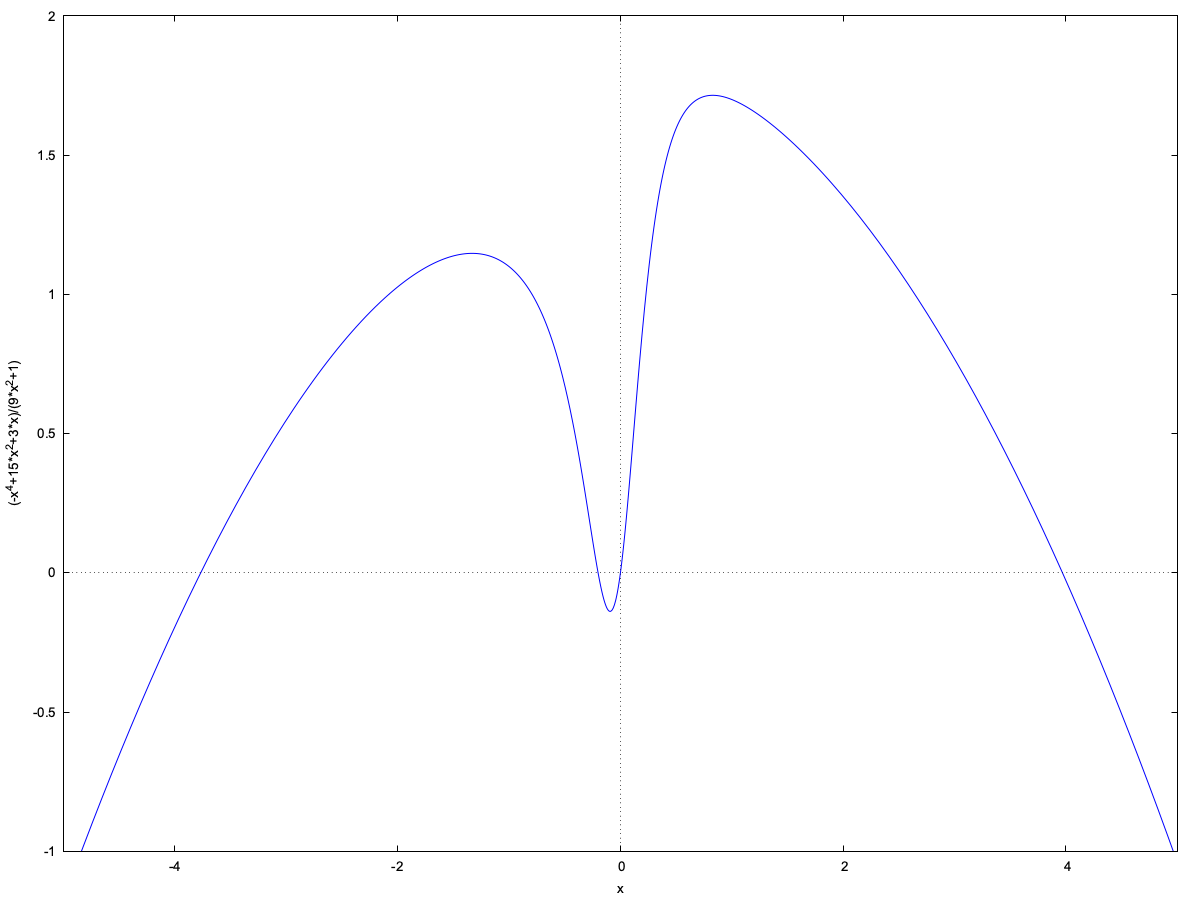
\includegraphics[width=.95\linewidth,height=.80\textheight,keepaspectratio]{quesrtion_7_img/quesrtion_7_1}\mbox{}\]

\[\tag{\% o31} 
\mbox{}
\]
%%%%%%%%%%%%%%%%
b)


\noindent
%%%%%%%%
%% INPUT:
\begin{minipage}[t]{4.000000em}\color{red}\bfseries
(\% i32)	
\end{minipage}
\begin{minipage}[t]{\textwidth}\color{blue}
diff(f(x),x);
\end{minipage}
%%%% OUTPUT:
\[\displaystyle \tag{\% o32} 
\frac{\mathop{-}\left( 4 {{x}^{3}}\right) \mathop{+}30 x\mathop{+}3}{9 {{x}^{2}}\mathop{+}1}\mathop{-}\frac{18 x\, \left( \mathop{-}{{x}^{4}}\mathop{+}15 {{x}^{2}}\mathop{+}3 x\right) }{{{\left( 9 {{x}^{2}}\mathop{+}1\right) }^{2}}}\mbox{}
\]
%%%%%%%%%%%%%%%%
c)


\noindent
%%%%%%%%
%% INPUT:
\begin{minipage}[t]{4.000000em}\color{red}\bfseries
(\% i76)	
\end{minipage}
\begin{minipage}[t]{\textwidth}\color{blue}
ratsimp(df(x):=''(diff(f(x),x)));
\end{minipage}
%%%% OUTPUT:
\[\displaystyle \tag{\% o76} 
\mathop{df}(x)\mathop{:=}\mathop{-}\left( \frac{18 {{x}^{5}}\mathop{+}4 {{x}^{3}}\mathop{+}27 {{x}^{2}}\mathop{-}30 x\mathop{-}3}{81 {{x}^{4}}\mathop{+}18 {{x}^{2}}\mathop{+}1}\right) \mbox{}
\]
%%%%%%%%%%%%%%%%


\noindent
%%%%%%%%
%% INPUT:
\begin{minipage}[t]{4.000000em}\color{red}\bfseries
(\% i75)	
\end{minipage}
\begin{minipage}[t]{\textwidth}\color{blue}
ratsimp(ddf(x)\ :=\ ''(diff(df(x),\ x)));\\

\end{minipage}
%%%% OUTPUT:
\[\displaystyle \tag{\% o75} 
\mathop{ddf}(x)\mathop{:=}\mathop{-
}\left( \frac{162 {{x}^{6}}\mathop{+}54 {{x}^{4}}\mathop{-}486 {{x}^{3}}\mathop{+}822 {{x}^{2}}\mathop{+}162 x\mathop{-}30}{729 {{x}^{6}}\mathop{+}243 {{x}^{4}}\mathop{+}27 {{x}^{2}}\mathop{+}1}\right) \mbox{}
\]
%%%%%%%%%%%%%%%%


\noindent
%%%%%%%%
%% INPUT:
\begin{minipage}[t]{4.000000em}\color{red}\bfseries
(\% i44)	
\end{minipage}
\begin{minipage}[t]{\textwidth}\color{blue}
solve(df(x)\ =\ 0,\ [x,y]);
\end{minipage}
%%%% OUTPUT:
\[\displaystyle \tag{\% o44} 
\mathop{[}\left[ x\mathop{=}0.298\mathop{-}1.24 \% i\mathop{,}y\mathop{=}\ensuremath{\mathrm{\% r31}}\right] \mathop{,
}\left[ x\mathop{=}1.24 \% i\mathop{+}0.298\mathop{,}y\mathop{=}\ensuremath{\mathrm{\% r32}}\right] \mathop{,
}\left[ x\mathop{=}0.829\mathop{,}y\mathop{=}\ensuremath{\mathrm{\% r33}}\right] \mathop{,}\left[ x\mathop{=}\mathop{-}1.33\mathop{,}y\mathop{=}\ensuremath{\mathrm{\% r34}}\right] \mathop{,
}\left[ x\mathop{=}\mathop{-}0.0924\mathop{,}y\mathop{=}\ensuremath{\mathrm{\% r35}}\right] \mathop{]}\mbox{}
\]
%%%%%%%%%%%%%%%%


\noindent
%%%%%%%%
%% INPUT:
\begin{minipage}[t]{4.000000em}\color{red}\bfseries
(\% i39)	
\end{minipage}
\begin{minipage}[t]{\textwidth}\color{blue}
ddf(0.829);
\end{minipage}
%%%% OUTPUT:
\[\displaystyle \tag{\% o39} 
\mathop{-}1.27\mbox{}
\]
%%%%%%%%%%%%%%%%
As ddf(x) at this point is \ensuremath{<}0 this is a maximum


\noindent
%%%%%%%%
%% INPUT:
\begin{minipage}[t]{4.000000em}\color{red}\bfseries
(\% i22)	
\end{minipage}
\begin{minipage}[t]{\textwidth}\color{blue}
realroots(18*x\^\ 5\ +\ 4*x\^\ 3\ +\ 27*x\^\ 2\ -\ 30*x\ -\ 3);\\

\end{minipage}
%%%% OUTPUT:
\[\displaystyle \tag{\% o22} 
\left[ x\mathop{=}\mathop{-}\left( \frac{44684171}{33554432}\right) \mathop{,}x\mathop{=}\mathop{-}\left( \frac{3101157}{33554432}\right) \mathop{,}x\mathop{=
}\]\[\frac{27810445}{33554432}\right] \mbox{}
\]
%%%%%%%%%%%%%%%%


\noindent
%%%%%%%%
%% INPUT:
\begin{minipage}[t]{4.000000em}\color{red}\bfseries
(\% i47)	
\end{minipage}
\begin{minipage}[t]{\textwidth}\color{blue}
pos\_root:\ find\_root(18*x\^\ 5\ +\ 4*x\^\ 3\ +\ 27*x\^\ 2\ -\ 30*x\ -\ 3,\ x,\ 0,\ 6);\\

\end{minipage}
%%%% OUTPUT:
\[\displaystyle \tag{pos\_ root} 
0.829\mbox{}
\]
%%%%%%%%%%%%%%%%


\noindent
%%%%%%%%
%% INPUT:
\begin{minipage}[t]{4.000000em}\color{red}\bfseries
(\% i45)	
\end{minipage}
\begin{minipage}[t]{\textwidth}\color{blue}
f(pos\_root);\\

\end{minipage}
%%%% OUTPUT:
\[\displaystyle \tag{\% o45} 
1.72\mbox{}
\]
%%%%%%%%%%%%%%%%


\noindent
%%%%%%%%
%% INPUT:
\begin{minipage}[t]{4.000000em}\color{red}\bfseries
 --\ensuremath{\ensuremath{>}}	
\end{minipage}
\begin{minipage}[t]{\textwidth}\color{blue}
f(\%o60);
\end{minipage}
%%%% OUTPUT:
\[\displaystyle \tag{\% o66} 
\mathop{[}\frac{\mathop{-
}\]\[{{x}^{4}}\mathop{+
}\]\[15\]\[{{x}^{2}}\mathop{+
}\]\[3 x}{9\]\[{{x}^{2}}\mathop{+
}\]\[1}\mathop{=}1.147\mathop{,}\frac{\mathop{-
}\]\[{{x}^{4}}\mathop{+
}\]\[15\]\[{{x}^{2}}\mathop{+
}\]\[3 x}{9\]\[{{x}^{2}}\mathop{+
}\]\[1}\mathop{=}\mathop{-
}0.1386\mathop{,}\frac{\mathop{-
}\]\[{{x}^{4}}\mathop{+
}\]\[15\]\[{{x}^{2}}\mathop{+
}\]\[3 x}{9\]\[{{x}^{2}}\mathop{+
}\]\[1}\mathop{=}1.715\mathop{]}\mbox{}
\]
%%%%%%%%%%%%%%%%


\noindent
%%%%%%%%
%% INPUT:
\begin{minipage}[t]{4.000000em}\color{red}\bfseries
(\% i62)	
\end{minipage}
\begin{minipage}[t]{\textwidth}\color{blue}
float(find\_root(f(x),x,0,6));
\end{minipage}
%%%% OUTPUT:
\[\displaystyle \tag{\% o62} 
0.0\mbox{}
\]
%%%%%%%%%%%%%%%%


\noindent
%%%%%%%%
%% INPUT:
\begin{minipage}[t]{4.000000em}\color{red}\bfseries
(\% i58)	
\end{minipage}
\begin{minipage}[t]{\textwidth}\color{blue}
find(f(x),\ x,\ 0,\ 6);
\end{minipage}
%%%% OUTPUT:
\[\displaystyle \tag{\% o58} 
0.0\mbox{}
\]
%%%%%%%%%%%%%%%%


\noindent
%%%%%%%%
%% INPUT:
\begin{minipage}[t]{4.000000em}\color{red}\bfseries
(\% i73)	
\end{minipage}
\begin{minipage}[t]{\textwidth}\color{blue}
quad\_qags(f(x),x,0,3.97);
\end{minipage}
%%%% OUTPUT:
\[\displaystyle \tag{\% o73} 
\left[ 4.34\mathop{,}2.63 {{10}^{-9}}\mathop{,}105\mathop{,}0\right] \mbox{}
\]
%%%%%%%%%%%%%%%%


\noindent
%%%%%%%%
%% INPUT:
\begin{minipage}[t]{4.000000em}\color{red}\bfseries
(\% i77)	
\end{minipage}
\begin{minipage}[t]{\textwidth}\color{blue}
integrate(f(x),x,0,3.969);
\end{minipage}
%%%% OUTPUT:
\[\displaystyle rat: replaced 3.97 by 3969/1000 = 3.97
rat: replaced 3.97 by 3969/1000 = 3.97
rat: replaced 3.97 by 3969/1000 = 3.97
rat: replaced 3.97 by 3969/1000 = 3.97
rat: replaced 3.97 by 3969/1000 = 3.97
rat: replaced 3.97 by 3969/1000 = 3.97
rat: replaced 3.97 by 3969/1000 = 3.97
rat: replaced 3.97 by 3969/1000 = 3.97
rat: replaced 3.97 by 3969/1000 = 3.97
rat: replaced 3.97 by 3969/1000 = 3.97
rat: replaced 11.9 by 11907/1000 = 11.9
rat: replaced 3.97 by 3969/1000 = 3.97
\mbox{}\]

\[\tag{\% o77} 
0.167 \log{\left( \frac{142776649}{1000000}\right) }\mathop{-}0.56 \operatorname{atan}{\left( \frac{11907}{1000}\right) }\mathop{+}4.35\mbox{}
\]
%%%%%%%%%%%%%%%%
\end{document}
